\section{Results and Tests}


\subsection{uClinux}
After building and flashing \emph{uClinux} on the chip, we verified that we had a working Linux distribution by connecting to its shell with \emph{miniterm.py} and running Linux commands like \emph{ls} and \emph{cat}. In addition to this, we saw Tux on the screen, indicating that \emph{uClinux} was properly installed.

\subsection{Gamepad driver}
\begin{figure}[h]
	\centering
	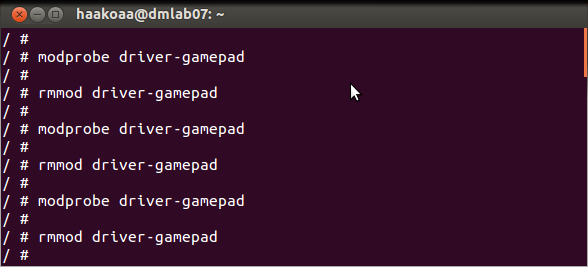
\includegraphics[width=12cm]{img/modprobe.png}
	\caption{Adding and removing the module several times}
	\label{fig:modprobe}
\end{figure}
Testing that the gamepad driver delivers the correct data to the user space is left to our game. If the game functions as expected, we can therefore conclude that the gamepad driver reads and delivers the correct data. Please read on (section \ref{subsection:pong-testing}) to verify the correctness of this.\\
\\
In addition to delivering the correct data on time, it is really important that the driver cleans up properly by deallocating and freeing various data structures used for it's operation. Failing to do so, might cause memory leaks in kernel space; a situation where memory does not get freed before system reboot. Besides from being very accurate (making sure each allocation call had a corresponding deallocation call) in writing the drivers probe and close functions, we tested that we were able to load and uload our kernel module multiple times. We did a test by calling \emph{modprobe driver-gamepad} and \emph{rmmod driver-gamepad} consecutively three times, checking that neither of the calls yielded any error messages. As we can see in figure \ref{fig:modprobe}, the test was a success.

\subsection{Pong}
\label{subsection:pong-testing}
When designing a game, user experience is everything, and it is important that the system behaves as expected. In particular, we focused on the following aspects:

\paragraph{Game behaviour}
The game should follow the rules of pong. In particular:
\begin{itemize}
	\item The ball should bounce off the player paddles, in addition to the upper and lower walls.
	\item If a player miss the ball, the game should reset.
	\item Up and down buttons on each controller should control the corresponding player paddle. The paddle should move as long the button is pressed down, as long it is within it's legal horizontal bounds.
\end{itemize}

\paragraph{Performance}
The game speed should never reduce and the frame update rate should stay at 24 FPS. No player interaction should exhaust the computation resources of the chip, making the game slower. We did no scientific way of measuring the frames per seconds, but the animations are not adjusted after the given FPS. When a player notices a speed reduce in the game, we can therefore conclude that the FPS has been lowered.

\paragraph{No rendering artifacts}
No artifacts with the elements drawn on the screen should appear. By that, we mean that all rectangular shapes should stay in the same color and shape during the game. An example of unwanted behaviour is shown in figure \ref{fig:pong_overlapping}, where the ball removes some pixels from the paddle. In addition to this, no flickering of any screen elements should be present. \\
\\
The game behaviour was tested by playing the game over and over (the game is actually quite entertaining) looking for unexpected behaviour. We confirmed that the game behaved as expected, with one minor flaw: The player movement has unintuitive behaviour if two buttons are pressed at the same time. If up is pressed while down is already pressed, the paddle will move up, but when up is released again, the paddle will stop moving. The most intuitive behaviour would be to let the paddle move down, as the down button is pressed. We decided to not fix this issue, because it requires extra book-keeping in the application, in addition to the very simple solution: Don't press up and down at the same time.\\
\\
Testing performance and rendering has very much to do with the next section, where we will elaborate on different rendering modes.

\subsection{Energy efficiency and performance}
\begin{table}
	\begin{tabular}{c|c|c}
		\hline
		\hline
		& Test 1 & Test 2\\
		\hline
		Single & $11.87mA$ & $12.38mA$ \\
		Double & $11.94mA$ & $12.37mA$ \\
		Full & $31.82mA$ & $31.93mA$ \\
		Tickless & $11.46mA$ & $11.98mA$ \\
		\hline
		
	
	\end{tabular}
\end{table}

\subsubsection{Performance and energy efficiency with different frame update modes}

\subsubsection{Tickless idle}

\subsection{Further development}
\paragraph{Memory Mapping}
Memory mapping is a technique used to transfer data between kernel space and userspace without copying. It is the fastest way to handle larger amount of data. The screen module uses this technique when writing to the framebuffer. We thought our driver could benefit from offering a way to use mmap to read the values of the buttons pressed. We attempted to create open and close functions for mmap and assign them to their respective fields in the \emph{vm\_operations} struct. Also a \emph{fault} function where created, wich seems to be the inheritor after the \emph{nopage} got removed. Lastly a function to assign the file data to the virtual memory data where created and assigned to the \emph{mmap} field of the \emph{file\_operations} struct. We failed however to get this to work (, wich is why it is described here and not in the \emph{description of methology} section). It seemed like the \emph{mmap} fuction never got called. Benjamin, who also thought it would be nice of our driver to support memory mapping, where helpfull but unsucessfull when trying to find the problem with us. He did however come with some suggestions where to look for clues, such as in the source code of the framebuffer. As it was not part of the assignment, and since we felt that it had allready taken to much of our time, we did not proceed with any further investigations at this point.
